\section{Study 1: Policies}\label{sec:personality:study-1}
% general motivation - why do we investigate this?
We start out with the exploration of psychological factors for the design of password policies. We were motivated by the fact that, at this point, policies are a one-fits-all solution that evidently does not work in the same ways for all users: Shay \etal observed that subjective usability ratings for policies differed among participants \cite{Shay2012CorrectHorseBatteryStaple, Shay2014CanLongPasswordsBeSecureAndUsable}. For instance, about 40\% of their participants found it difficult to create a password under a ``3class16'' policy, but another 40\% found it easy \cite{Shay2014CanLongPasswordsBeSecureAndUsable}. Following the general discourse and related results from privacy research, we hypothesized that an individual's personality might be responsible for their attitudes towards one policy or another. Therefore, our goal in this project was to explore such associations between personality traits and policy preference. At this point, we leave out analyses on password strength.
%GOALS: explore associations between big-five traits and password selection under different policies, both on usability and security metrics. Investigate the effects of using a non-traditional password policy based on emojis. user preference for one policy or another. explorative study so no p-values.
\subsection{Method}
% general methodology
Our study was completely exploratory, because the literature did not allow us to derive narrow hypotheses. Since personality traits are nuanced, we opted for an online survey to collect a large sample. Personality was assessed based on the Five-Factor Model. We opted for the very reliable BFI-K construct by Rammstedt and John \cite{Rammstedt2005BFI}, which is also freely available in German. Moreover, with its 21 items, the time to fill out the questionnaire is kept reasonably low. 
Participants were asked to create several passwords in a row, i.e. the study followed a within-groups protocol. Here, we evaluated three different password policies: a traditional (3class12), an uncommon (2word12), and a novel policy (emoji12) that required the selection of at least one emoji through a graphical user interface (more on emojis in Chapter \ref{chap:emojipasswords}). The reason for this choice was that the policies are different enough to serve as characteristic levels of the independent variable ``policy''. Participants assessed the ``difficulty to create'' of a password for each policy. Moreover, we had them rank the policies by their personal preference, so the distinctiveness of 3class12, 2word12, and emoji12 would help them spot and judge the differences easily, which makes the data more reliable.

\subsubsection{Structure and Tasks}
The study was divided into 3 overall parts. In the first part, participants were briefed about privacy details of the study and they provided demographic background information. Then they proceeded to the personality questionnaire before they were asked to perform three experimental tasks. Each consisted of creating a password and assessing the difficulty with agreement levels on the three items \textit{``It was difficult to create a password that meets the requirements''}, \textit{``I found the password requirements bothersome''}, and \textit{``It was easy to create a \textit{new} password''}. Agreement was measured on a five-point scale ranging from ``Strongly disagree'' to ``Strongly agree''. Inversely keying the items as well double encoding makes the data more robust against implausible responses. The resulting difficulty-to-create score thus ranges from 3 to 15 (3 = very easy, 15 = very difficult).

The order of the policies was counterbalanced during the experiment to mitigate order effects. For each participant, we recorded the resulting order as a control variable. We chose an online-banking scenario for all three selection tasks. The first prompt was to create a password to protect an online banking account. Secondly, participants were told that someone had gained access to their account and the bank locked them out. As a security precaution, they had to reset their first password. The last task description explained that their password had expired after one year and they need to reset it again. This storyline was designed to fulfill the \textit{realistic threat} principle proposed by Krol \etal (see Section \ref{sec:rw:principles-experiments}) \cite{Krol2016ExperimentDesign}. 

We used SosciSurvey, a standard survey tool, to collect the responses. The dynamic parts involving password selection were embedded in iframes. To match the data from the survey tool and the iframe we used URL query parameters containing the response ID. We asked participants to only use a desktop browser to avoid styling glitches and unexpected behavior from the prototypes. %Auto-complete was prevented in any case

\subsubsection{Recruiting and Demographic Background}
We recruited participants through posts on social networks and by sending out the invitation link in a university-wide newsletter (more than 5000 recipients). To incentivize participation, we announced a raffle of five shopping vouchers with a value of 20€ each. At this point, 222 people had started participation. After drop-out and plausibility checks, the remaining sample size was $N=164$. As expected, the age distribution was narrow: our sample consisted mostly of students in their mid-twenties (average age 24 (SD=5). 79 respondents were female, 83 male, and 2 preferred not to answer. In the background screener, 65 people (40\%) indicated to possess formal training in computer science or information technology. We also requested self-reported assessments on password practices. Here we found that 40\% reuse passwords without modification, 32\% reuse them with modifications or with a mnemnoic technique. 17\% often create new passwords. In terms of management strategy, the majority (53\%) tries to memorize passwords. 11\% use a password manager or generator. Written cues served as aid for 10\% of respondents, and 16\% write passwords down on analog media, while 21\% use electronic files. Interestingly, the distribution of coping strategies is very close to survey findings gathered with more diverse samples \cite{CSID2012PasswordHabits}. Hence, we believe to have caught a representative snapshot of password behavior.

\subsubsection{Statistical Analyses}
For statistical analyses, we consulted the StabLab\footurl{http://www.stablab.stat.uni-muenchen.de/}{30.01.2018} to identify suitable methods. After a revision of the collected data and the necessary assumption checks, we analyzed associations by fitting \glspl{GAM} to the dataset. Their advantage over linear regression is that they are more flexible for non-linear associations\footurl{https://en.wikipedia.org/wiki/Additive_model}{30.01.2018}. The \textit{mgcv} package for R was used to calculate the models. GAMs can be primarily interpreted through residual/smooth plots -- the steeper the fitted regression line, the stronger the association (The box in the results section  (\ref{sec:personality:how-to-read-gam}) explains how to read GAM plots in great detail.)

Scores on the Big-Five sub-dimensions served as independent variables, i.e. the predictors in the regression models. \textit{Openness} is coded with five items, while the remaining four dimensions were assessed with four items each. The agreement level for every item was mapped to numeric values from 1 to 5. The score on each sub-dimension is the sum of agreement levels. To better estimate effect sizes, we control for gender, age and IT proficiency in the regression models. 

\subsubsection{Method Limitations}
The method, albeit carefully executed, faces a few limitations regarding the interpretability of the data. First, the sample was fairly homogeneous, because participants were mostly between 20 and 28 years old and have an academic background. This might reduce statistical power in detecting effects on personality \cite{Srivastava2003PersonalityAdulthood}, but on the other hand, this constellation resolves age-related confounding effects. Moreover, our study was strongly focused on individual preferences and usability perceptions of different policies, so only a within-groups design was feasible. However, in real-life password selection, users rarely select three passwords in a row. The choice of our storyline still makes us confident about the ecological validity \cite{Fahl2013EcologicalValidityPasswordStudy}. The repeated measures design did not allow us to measure the policies' influence on password memorability, which we have to postpone to another study. At this stage, the subjective preference was more valuable for our exploration than memorability effects. Besides, we briefed participants to fill out the survey on a desktop PC or a similar device. We cannot guarantee that all participants followed this instruction, which might have had an effect on their password selection \cite{Melicher2016UsabilityMobileTextPasswords}. 

% we had to redeploy the prototype.
Finally, we unfortunately made a mistake in the deployment of the emoji-based policy. Instead of 12 characters, it required participants to select 16 characters beside the emoji. We realized this fact by looking at descriptive statistics during the course of the study, because the policy performed significantly worse than the other two. We re-deployed the emoji-based policy immediately after we had realized the error. Consequently, we had to remove the data for the creation difficulty and ranking in cases 1-61, reducing the overall sample size to 103. Nonetheless, the sample size is sufficiently large to investigate medium to strong effects. 

%- we started out with emoji16, but made the switch to emoji12 (after 43 participants), because emoji16 received the most negative feedback, but it was mostly due to the length. data removed for ranking (1-61) and difficulty to create (1-43). 

%%%%%%%%%%%
%%%%%%%%%%%
%%%%%%%%%%% Results
%%%%%%%%%%%
\subsection{Results}
Overall, associations between personality and policies were moderate. In the following, we only describe non-trivial and interesting associations. 

\begin{figure}[htbp]
	\centering
	\begin{subfigure}[t]{0.49\linewidth}
		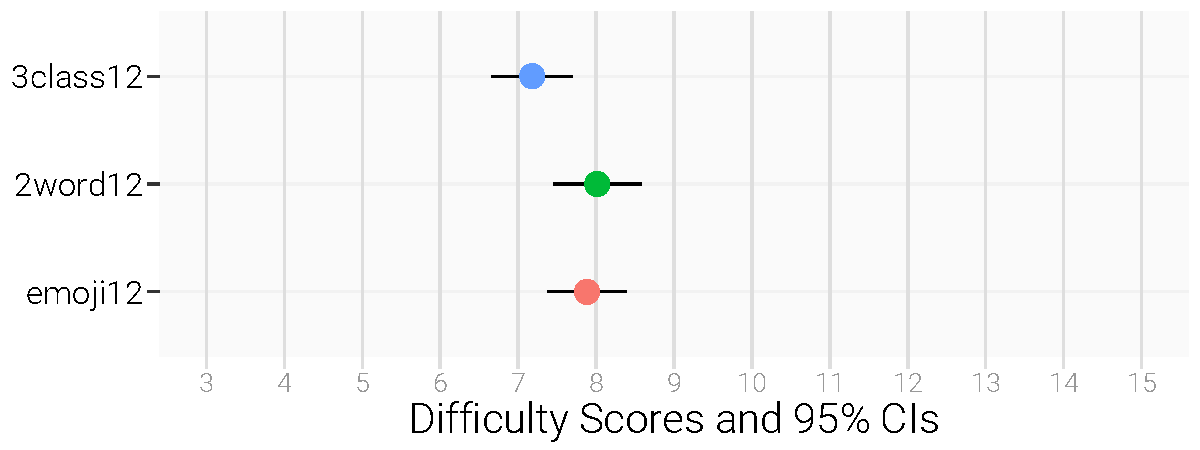
\includegraphics[width=\textwidth]{personality/difficulty-ci}
		\caption{\label{fig:personality:study-1-difficulty-ci}}
	\end{subfigure}
	\begin{subfigure}[t]{0.49\linewidth}
		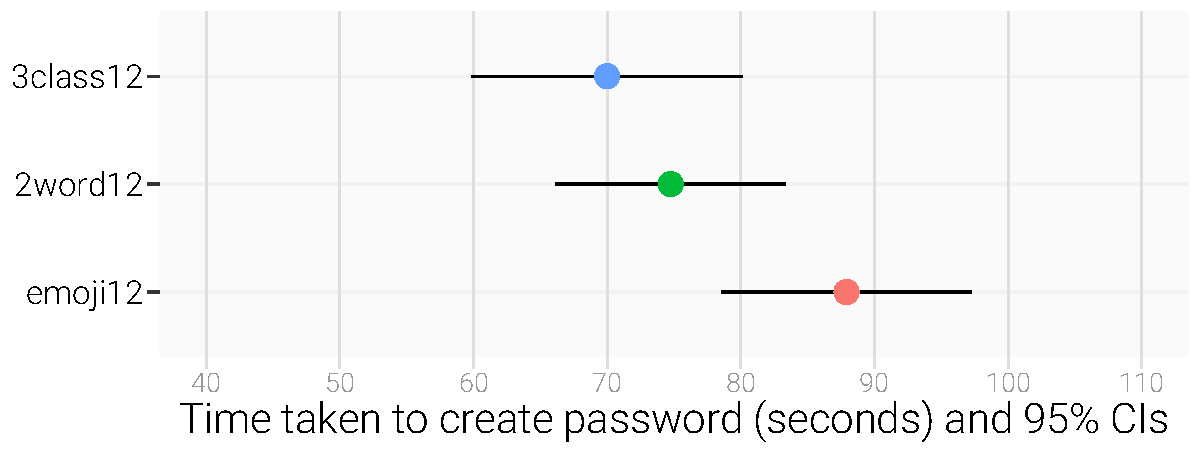
\includegraphics[width=\textwidth]{personality/timing-ci}
		\caption{\label{fig:personality:study-1-timing-ci}}
	\end{subfigure}
	\caption{\label{fig:personality:study-1-usability-stats}Confidence Intervals for a) Difficulty to create and b) time to create passwords in each condition. The traditional policy (3class12) was the easiest and fastest overall, but not on a statistically significant level (also visible in the charts due to the overlapping confidence intervals)}
\end{figure}
\subsubsection{Descriptives and Independent Variables}
Users rated the difficulty to create a password very similarly in all conditions (averages of scores in range [3;15]: 3class12 = 7.18, 2word12 = 8.02, emoji12 = 7.88). A linear mixed model ANOVA did not show significant differences (\statsgt{2+2}{5.28}{0.1}). Figure \ref{fig:personality:study-1-usability-stats} shows the confidence intervals for these two usability metrics ``difficulty to create'' and ``time to create''. Observing no significant differences overall is interesting because it means that individual ratings could be explained by personality traits. %TODO that's not quite clear.



%serial positioning effects do make a difference, but it also appears trivial in the overall sample.
%summary: no big difference between policies and ranking. (this is what makes the remainder more exciting, because a %closer look at the data brings out how the numbers come to be)

%%%%%%%%%%%
%%%%%%%%%%% Difficulty to create a password with a given policy
%%%%%%%%%%%
\subsubsection{Creation Difficulty Models}
The general additive models showed associations between the predictors and creation difficulty scores (see Table \ref{tab:personality:study-1-coffections-clean}). 
\begin{table}[htbp]
  \centering
    \begin{tabular}{l|SS|SS|SS}
          & \multicolumn{2}{c|}{\textit{emoji12}} & \multicolumn{2}{c|}{\textit{2word12}} & \multicolumn{2}{c}{\textit{3class12}} \\ \hline \hline
          (Intercept) & \multicolumn{2}{c|}{$9.99$} & \multicolumn{2}{c|}{$7.04$} & \multicolumn{2}{c}{$6.26$} \\ \hline
\multicolumn{1}{c|}{Predictor}  & \multicolumn{1}{c}{$\beta$} & \multicolumn{1}{c|}{$\sigma_n$} & \multicolumn{1}{c}{$\beta$} & \multicolumn{1}{c|}{$\sigma_n$} & \multicolumn{1}{c}{$\beta$} & \multicolumn{1}{c}{$\sigma_n$}  \\
    Age & 0.02  & 0.06  &       &       & -0.05 & 0.06 \\
    Gender (female) & 0.91  & 0.58  & 1.35  & 0.66  & -0.46 & 0.61 \\
    No IT Background & -0.10 & 0.59  & 0.60  & 0.66  & 0.21  & 0.63 \\
    Extraversion & -0.05 & 0.08  &       &       & -0.01 & 0.08 \\
    Conscientiounsness & 0.01  & 0.09  &       &       & 0.08  & 0.10 \\
    Neuroticism & -0.22 & 0.09  &       &       & 0.05  & 0.09 \\
    \textit{emoji12} Position 2 & 0.52  & 0.65  &       &       &       &  \\
    \textit{emoji12} Position 3 & 0.23  & 0.63  &       &       &       &  \\
    \textit{2word12} Position 2 &       &       & -0.38 & 0.74  &       &  \\
    \textit{2word12} Position 3 &       &       & -0.07 & 0.73  &       &  \\
    \textit{3class12} Position 2 &       &       &       &       & 1.19  & 0.66 \\
    \textit{3class12} Position 3 &       &       &       &       & 0.77  & 0.69 \\ \hline
%    edf: s(Age) & \multicolumn{2}{c|}{} & \multicolumn{2}{c|}{1.81} & \multicolumn{2}{c}{} \\
%    edf: s(Agreeableness) & \multicolumn{2}{c|}{3.27} & \multicolumn{2}{c|}{2.77} & \multicolumn{2}{c}{2.02} \\
%    edf: s(Openess) & \multicolumn{2}{c|}{2.50} & \multicolumn{2}{c|}{1.79} & \multicolumn{2}{c}{1.53} \\
%    edf: s(Extraversion) & \multicolumn{2}{c|}{} & \multicolumn{2}{c|}{1.52} & \multicolumn{2}{c}{} \\
%    edf: s(Conscientiousness) & \multicolumn{2}{c|}{} & \multicolumn{2}{c|}{3.32} & \multicolumn{2}{c}{} \\
%    edf: s(Neuroticism) & \multicolumn{2}{c|}{} & \multicolumn{2}{c|}{1.53} & \multicolumn{2}{c}{} \\ \hline
    Explained Deviance & \multicolumn{2}{c|}{0.15} & \multicolumn{2}{c|}{0.21} & \multicolumn{2}{c}{0.10} \\
    Num. Observations. & \multicolumn{2}{c|}{119} & \multicolumn{2}{c|}{119} & \multicolumn{2}{c}{119} \\
    Num. Smooth terms & \multicolumn{2}{c|}{2} & \multicolumn{2}{c|}{6} & \multicolumn{2}{c}{2} \\\hline
    \multicolumn{7}{l}{\textit{Description:}} \\ 
    \multicolumn{7}{l}{$\beta$ = Correlation coefficient} \\
    \multicolumn{7}{l}{$\sigma_n$ = standard error} \\
    \multicolumn{7}{l}{edf = estimated degrees of freedom by non-linear effects} \\
    \multicolumn{7}{l}{(\glqq estimated degrees of freedom\grqq)} \\
    \multicolumn{7}{l}{Smooth terms = non-linear effects in the model} \\
    \end{tabular}%
  \caption{Additive regression models for the difficulty to create passwords under the three policies.}
\label{tab:personality:study-1-coffections-clean}
\end{table}%
\paragraph{Control Variables} 
The GAM allowed us to model associations linearly for the control variables (example for emoj12 in Figure \ref{fig:personality:dc-emoji-b5}). Although we have to be careful not to generalize too strongly with our sample, linear associations at least enable us to use correlation coefficients $B$ as basis for discussion.
% gender
Female participants assessed it slightly more difficult to create passwords under the emoji12 ($B=0.91$) and 2word12 ($B=1.35, p<0.05$) policies than male participants. For 3class12, the correlation was smaller ($B=-0.46$) and pointed in the opposite direction. 
% it background
Having a background in IT positively showed medium correlations with difficulty in the 2word12 policy, too ($B=0.61$). This policy, albeit alphanumeric, is uncommon in the wild and ignores the verdict of high complexity -- IT people might be skeptical about the ``words'' requirement, while others are less concerned about it.
% order of the policy
The task order also showed medium-strong influence on creation difficulty. If emoji12 or 3class12 were part of the second task, creation was seen as more difficult ($B_{emoij12-pos2}=0.52$),  ($B_{3class12-pos2}=1.19$). 
% age
% we observed non-linear associations between age and creation difficulty, but the small age range forbids us to make conclusive inferences from our data.

%, too: emoji12 ($B=-0.10$) trivial, 3class12 ($B=0.21$) weak, 2word12  medium. it looks as though people with higher IT knowledge struggle with a word-based policy, potentially because it is much less common in the wild. 

\begin{figure}
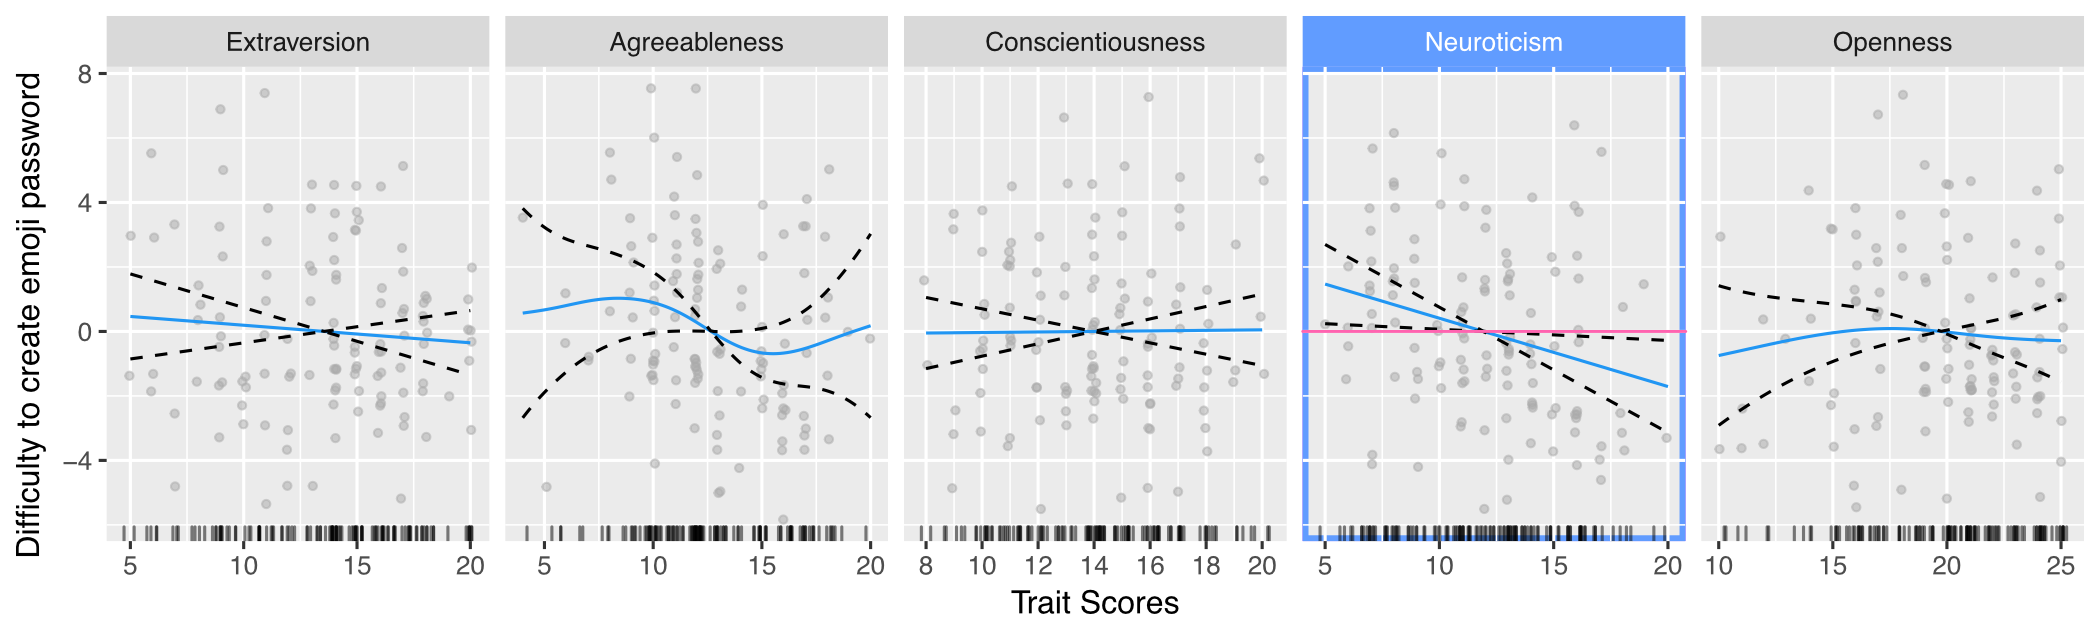
\includegraphics[width=\linewidth]{personality/dc-emoji-b5-v2}
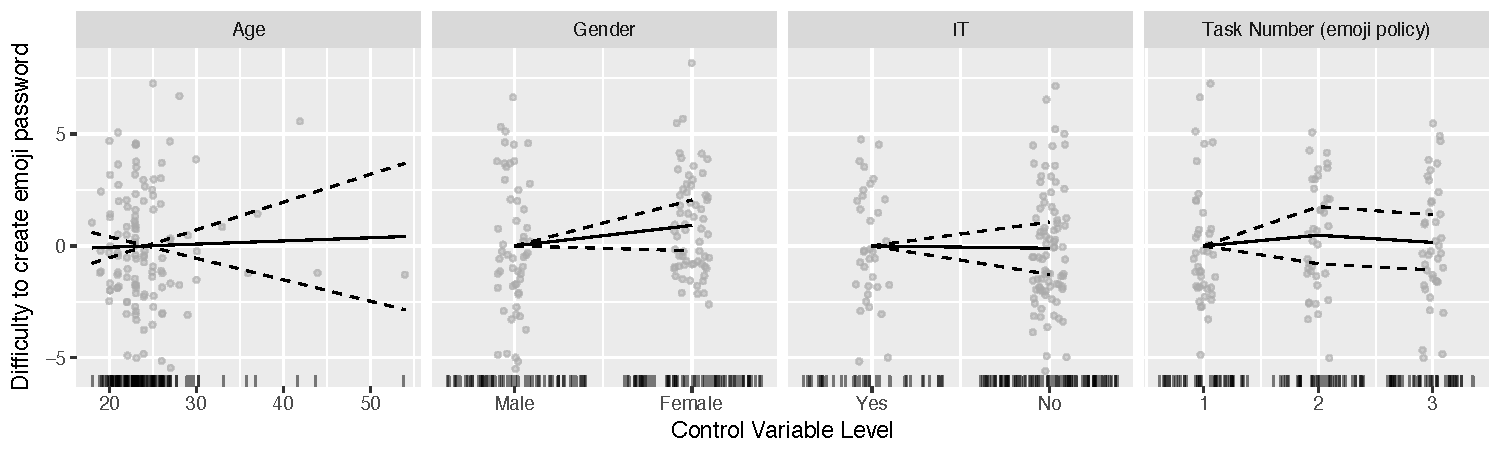
\includegraphics[width=\linewidth]{personality/dc-emoji-control-mod-v2}
\caption{\label{fig:personality:dc-emoji-b5}Associations between predictors and \textbf{difficulty} to create a password under the emoji12 policy. Charts visualize the functions derived from the Generalized Additive Models (GAMs). Neuroticism was significantly negatively associated with difficulty (highlighted in blue), i.e. it was easier to create emoji-passwords if participants scored high on neuroticism.}
\end{figure}

\noindent
\fbox{
	\label{sec:personality:study1:how-to-read-diagrams}
	\hspace{1cm}
	\centering
	\parbox[t][13cm]{0.85\linewidth}{
		\section*{How to Read Smoothed Regression Plots}\label{sec:personality:how-to-read-gam}
		Figure \ref{fig:personality:dc-emoji-b5} shows the first example of regression plots that will be used throughout the thesis where appropriate. There is a separate plot for each marginal association with a given predictor. The solid curve/line represents the estimated regression curve. If it is a straight line, the association can be modeled linearly (e.g. neuroticism in Figure \ref{fig:personality:dc-emoji-b5}). If it is a ``wiggly'' curve, the association is modeled with polynomial terms of different degrees (e.g. Agreeableness in Figure \ref{fig:personality:dc-emoji-b5}). The model intercept is at $y=0$. In many cases, residuals are plotted at their respective $(x,y)$ position to give a sense of clusters. At the bottom border of the plots, we often add ``rugs'' to show the number of observations/residuals along the x-axis. 
		
		Interpreting the effect size and significant contribution to the model fit is visible in two ways. First, the slope of the fitted line shows estimated strength of associations. Second, there are two dashed curves surrounding the fitted curve/line that visualize 95\% confidence intervals. Both curves are entirely above, respectively entirely below, the intersection between the fitted curve and the intercept at $y=0$, the association is significant at the 0.05 alpha level.
		
		In Figure \ref{fig:personality:dc-emoji-b5}, we highlighted this for the neuroticism plot. Left to the point of intersection, both dashed lines are above the intercept (in pink color); analogously, the dashed lines are below the intercept  on the right-hand side, indicating a significant contribution to the model. 
		
%		\begin{itemize}[leftmargin=*]
%			\item Personality is weakly associated with all the measured dimensions: strength perception, policy preference / usability, and password selection. Most notably openness and neuroticism showed conclusive associationes.
%			\item The models for the perception of passphrases achieved the highest fit, suggesting a predictable association between personality and strength perception for this type of password. Comparing two passwords was associated with the conscientiousness traits. Mixed models that use both password features and personality trait scores as covariates are the most feasible approach.
%			\item Older users might be the best target group for password support tools, because age was a good predictor of their usage. Suggesting good tools during account creation might lead to higher adoption 
%			%			\item Segmentation of users
%			\item Nudges designed for neuroticism should make emotional state more salient and highlight the benefits of \underline{long} passwords. 
%		\end{itemize}
	}
	\hspace{1cm}
}

\paragraph{Personality Traits}
Contrarily to the modeling functions for control variables, we mostly observed non-linear associations between trait scores and creation difficulty (see Figure \ref{fig:personality:dc-emoji-b5}).
%emoji personality
One exception is the weak linear association in the emoji12 ($B=-0.22$) condition. It tells us that it was slightly easier to create emoji-passwords for people with higher neuroticism scores. The neuroticism trait is also referred to as ``emotional stability'' \cite{Costa1992NEO}, i.e. neurotic people are usually more emotional. Expressing \textit{emotions} with emojis in passwords seems to support this trait and come easier to users scoring high on neuroticism. %(this is a great result, albeit weak. neurotic people are by defintion more \textit{emotional}, and emojis seem to cater to this trait.)

%agreeableness weak non linear, and interesting curve (up and down) for emoji12
%openness weak non linear, but too little data to conclusively decide. 

% 2word12 personality
%effects not as clear as for the emoji policy. highly open people report slightly less difficulty to create a 2word12 password.
In the models for the 2word12 policy, all associations were non-linear and thus inconclusive at this point. For the 3class12 policy, associations were linear but trivial for the extraversion, conscientiousness, and neuroticism factors. In summary, scores of the ``Creation Difficulty'' scale are difficult to explain with personality traits, but control variables appear to have stronger influence. Only neuroticism is associated notably with difficulty to create an emoji-password.
% 3class12
%linear associations are negligible for extraversion, conscientiousness, and neuroticism. 
%non-linear associations for agreeableness and openness. at value around 15 (from 20) the difficulty seems to increase (hard to interpret this finding). People with agreeableness scores of 18 and greater find it more difficult to create a 3class12 password by up to 1.5 points. Openness is inversely correlated here. the more open the participant was, the more likely they found it easy to create a 3class12 password. 

%%%%%%%%%%%
%%%%%%%%%%% Preference for one policy or another
%%%%%%%%%%%
\subsubsection{Policy Preference}
Table \ref{tab:pws_pers:distribution-binary-ranks} shows the overall preference for the three policies. It is evident that participants generally preferred the 3class12 policy (68\%). The emoji policy was best ranked by 18 participants, and 2word12 by 12 participants. Using logistic additive regression, we can determine the factors that contribute to these preferences. %https://web.stanford.edu/~hastie/Papers/AdditiveLogisticRegression/alr.pdf
In essence, the model gives us the likelihood of voting a given policy to the top, which is a binary decision (1 = preferred, 0 = not preferred). 
%did policy X land on top spot ? yes = 1, no = 1. thus, no encompasses the two other options.
%Logit model. 
\begin{table}
	\centering
	\caption{\label{tab:pws_pers:distribution-binary-ranks} Distribution of binary rankings of the three available policies. Evidently, 3class12 was ranked best in most cases. }
	\begin{tabular}{llll}
		~ 			& emoji12	& 2word12 	& 3class12 \\ \hline\hline
		1st rank	& 18		& 12		& 67 \\
		other rank 	& 80 		& 85 		& 31 \\ \hline
		n			& 98		& 98		& 98		 
	\end{tabular}
\end{table}

% predictors: demography and structure
Including demographic control variables as predictors, we observed strong effects for IT-background. The probability of putting emoji12 at the top is $exp(B{emoji-IT}) = 9.87$ for participants without technical background, so around ten times higher. Only one respondent with an IT background ranked emoji12 on the top. %This fits the finding that non-IT people found it easier to create an emoji12 password.
% order of policies 
The order in which policies were displayed also produced a notable effect. If emoji12 was part of the second $exp(B_{emoji-pos2}) = 0.27$ or third task $exp(B_{emoij-pos3}) = 0.76$, the likelihood to rate it the best policy slightly decreases. Other task orders, as well as age-related preferences, were inconclusive.

% personality
As with creation difficulty, rank-associations with personality traits were generally weak. The likelihood to prefer 2word12 decreased with higher extraversion scores $exp(B_{2word12-E}) = 0.82$. High agreeableness scores entailed higher chances to vote for emoji12 $exp(B_{emoji12-A}) = 1.28$. Interestingly, only very high neuroticism scores (>17) caused a  stark increase in favoring the emoji policy. However, the sample is thin in this area so the model is more unstable at this boundary. Other associations were negligible or inconclusive. 
%for agreeableness both linear and non-linear effects are visible; openness or conscientiousness have negligible, random associations. for neuroticism we lack data in edge cases (low or high trait scores) to draw conclusions. %there are more results in the BA, but I do not really see the point of reporting all the details of inconclusive results

%%%%%%%%%%%
%%%%%%%%%%% Password selection -- mostly emoji histogram
%%%%%%%%%%%
%\subsubsection{Password selection}

%\todo{create a emoiji selection histogram}. In essence, some emoji were strongly preferred, e.g. the red heart and the ``pouting face''. analyze: what were the usability ratings/rankings of those who picked the heart vs. the pouting face, i.e. are emojis with a positive connotation used by people who are happy that they can select an emoji password? I guess there are significant effects here. 

%TODO look into timings -- did conscientious people take longer to generate passwords?

\subsubsection{Time to Create Passwords}
The second usability metric was the time the participants took to create passwords. It can also be interpreted as \textit{effort} put into the task. The most interesting associations were visible for the 3class12 policy, where all personality traits could be modeled as linear predictors (see Figure \ref{fig:personality:timing-3class-b5}), and all showed medium-strong correlations (details in the Appendix, Table \ref{tab:personality:study-1:timing-models}). One might have suspected that conscientious people would invest more time, because one of their common attributes is diligence. However, this was not the case: conscientiousness was negatively associated with creation time for all policies ($B_{emoij12-C}=-3.58,B_{2word12-C}=-3.4,B_{3class12-C}=-2.09$). Neuroticism was significantly negatively associated with creation time, while agreeableness was marginally positively associated in 3class12. Demographic control factors indicated that, on average, women spent more time creating passwords in all conditions ($W=1166$, \pvallt{0.01}). The biggest effects were visible for task number as predictor: our participants took significantly less time to select passwords for the second and third tasks (example shown in \ref{fig:personality:timing-2word-control}). Most likely, this is a learning effect or due to people modifying their previous passwords. 


\begin{figure}
	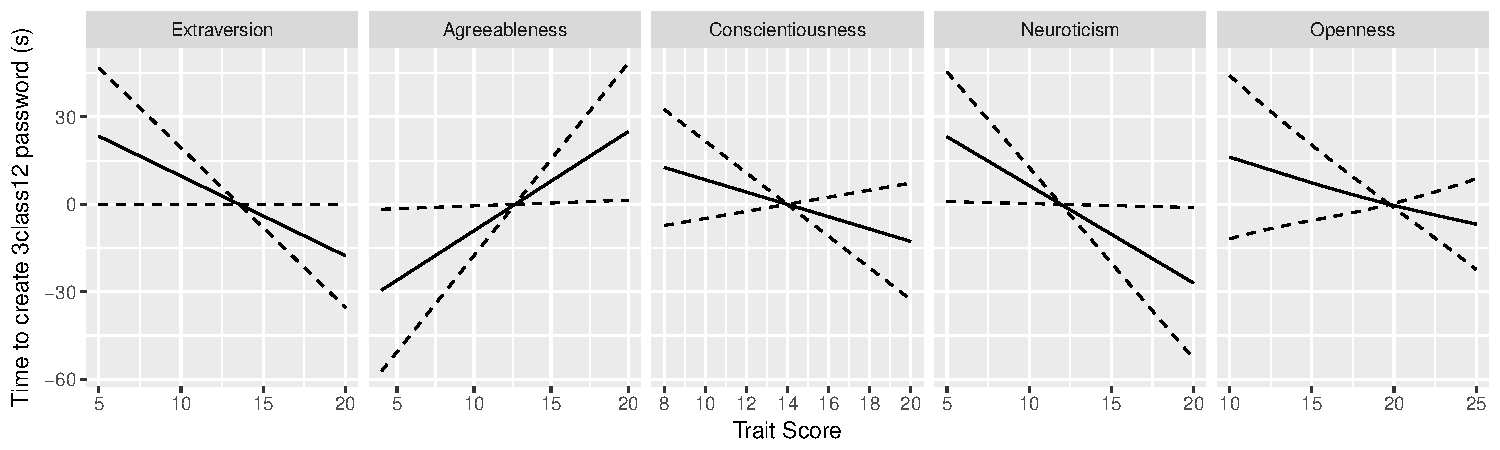
\includegraphics[width=\linewidth]{personality/timing-3class-b5}
	\caption{\label{fig:personality:timing-3class-b5}Associations between personality traits and time to create a 3class12 password. All traits could be modeled as linear predictors.}
\end{figure}

\begin{figure}
	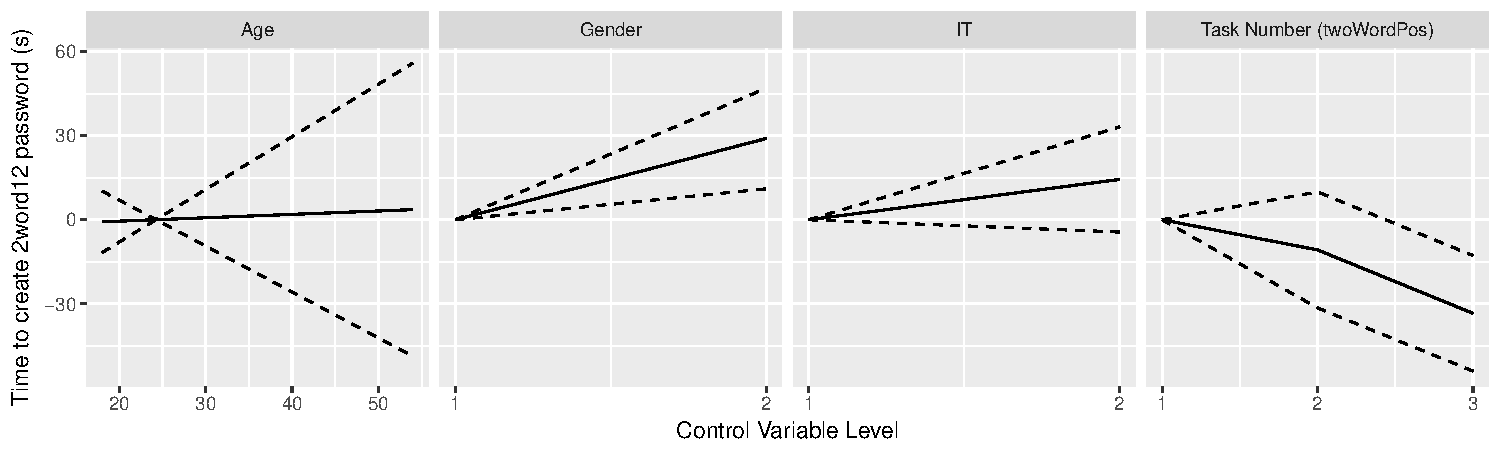
\includegraphics[width=\linewidth]{personality/timing-2word-control}
	\caption{\label{fig:personality:timing-2word-control}Associations between control variables and time to create a 2word12 password. Especially the task number and gender were showed strong associations.}
\end{figure}


%TODO the qualitative and plain-text passwords data is also interesting but goes too far at this point. 

\subsection{Finding Summary}
Overall, the usability metrics were comparable for all policies and the ranking was fairly homogeneous. So, any deviance from the mean could potentially be explained by personality traits and other confounding factors. In terms of personality, the most important finding was that scores on the neuroticism dimension seem to be positively associated with the usability of the emoji policy. As indicated above, emojis in passwords appear to fulfill their purpose in that they help some people express their emotions. Participants who did not have a background in IT were much more likely to prefer the emoji policy, and their neuroticism score played a subordinate role. Perhaps, a lack of expertise does not allow those participants to consider the switch from keyboard to mouse and vice versa (\textit{homing}). Moreover, the 3class12 policy received the most votes which might be due to the \textit{status quo bias} or \textit{familiarity bias}. 3class12 is the only commonplace policy among the tested ones, so participants were already used to it and voted it first. The timings were mostly affected by the task order -- participants spent less time on the second and third creation task. So although personality traits serve as predictors for timings, these effects were weaker by comparison. 

In summary, control factors had a greater effect on password usability and approval of policies than personality traits. Nonetheless, medium to strong effects are more likely to be detected with our sample size to begin with. So, the fact that we even observed small associations indicates that personality is a contributing factor to the perception of password policies. At this stage of the research we were not able to look into the selection behavior because the repeated measures design stood in the way. Thus, we designed and conducted two further studies to investigate the effect of personality on password strength perception and selection. 

%It could have been useful to include a recall test à la ``which passwords do you still remember after filling out the personality questionnaire?'' 

%medium associations between extraversion, agreeableness, and neuroticism (basically the other three dimensions that were not useful before), but control variables are associated to a larger degree.
%emoji policy similar results as traditional policies, i.e. it is wortwhile to experiment with it

%TODO re-read the discussion section, because the findings are a bit higher level and more understandable


%non linear associations probably explicable by other variables, e.g. intercorrelation -- 
%todo{discuss the personality traits and associations, try to explain them.}

%demographics play a role - (careful now, cowboy): policies could be tailored to gender. but i'm kind of reluctant to put this argument forward. at least IT background could be considered a factor for the policy. a personalized policy would make it more difficult for horizontal attacks because the policy is unpredictable.

%mutually exclusive effects for ranking are clear because of the binary nature.

%wild idea: if positioning influences the favorability of policies, one could leverage this. like anchoring and decoy (chose your own policy of the three). commitment and consistency as well (commit to your policy, create a strong password to be consistent with your commitment.)